\newpage
\section{مدل مورد استفاده در توسعه سیستم}
سیستمی که می‌خواهیم توسعه دهیم نیازمند فرایند های رفت و برگشتی بسیاری بین عوامل مختلف روند توسعه محصول هست. از ساعتی که پروژه شروع به توسعه می‌کند، 
نیازمندیم مرحله به مرحله کار ها رو به ترتیب اولویت انجام دهیم و به صورت چرخشی بازگردیم. برای مثال در نسخه اولیه که میخواهیم ارائه دهیم، دقیق نمیدانیم راهکار هایی که
در ذهن داریم، آیا جوابگو نیاز های کاربران هست یا خیر. از طرفی باگ ها و مشکلاتی در آینده وجود خواهند داشت که درحال حاضر از آنها بی اطلاع  هستیم.
جنبه های بیزینسی نیز کم نخواهند بود. به احتمال خیلی زیاد بعد از انتشار نسخه MVP ایراداد بیزینسی زیادی به پروژه وارد خواهد شد و این مشکلات به مرور زمان
در جلسات طراحی نرم افزار و بیزینس لاجیک باید صحبت بشوند. محصول نیاز به چندین بار طی کردن روند توسعه نرم افزار خواهد بود.

برای اینکه دقیق تر به موضوع بپردازیم، مرحله به مرحله قید خواهیم کرد. در مرحله اول، تیم UX باید تحقیق کنند که چه چیز هایی برای سیستم CRM ما نیاز هست.
باید ذی‌نفعان این محصول را شناسایی کرده و با تمامی آنها جلسه ای تنظیم کرد. پس از صحبت با آنها، می‌توان معماری بهتری چید.
برای مثال تیم محصول، حساب داری و فنی می‌توانند نظرات مفیدی را درمورد نیاز های خودشان بیان بکنند. این نظرات باید بایگانی شوند تا بعدا در جلسات طراحی برای 
رفع آنها فکر شود. البته در صورتی که درخواست ها منطقی باشند.
پس از آن تیم معماری نرم افزار (Architects) بر ساس یافته های خود شروع به چیدن یک سیستم می‌کنند.

بعد از مشخص شدن سیستم و شکوندن تسک ها و بستن اسپرینت توسط مدیر محصول، تیم های فنی دست به کار می‌شوند. توسعه دهنده ها شروع به نوشتند اجزا اصلی 
سیستم می‌کنند. تیم operation محیت لازم برای توسعه دهنده ها فراهم می‌کند.
تیم DevOps فرایند های اوتوماسیون لازم را می‌چیند و مهندسین تست انواع تست ها را مشخص می‌کنند.

نرم افزار داخل محیط تستی لانچ شده و تست می‌شود. بعد از گرفتن تائید واحد کنترل کیفیت، به مرحله بعد می‌رویم.

محصول بدست آمده به بازار ارزه می‌شود و بر اساس فیدبک ها و مشکلات گزارش شده تصمیم گرفته می‌شود که این چرخه ادامه داشته باشد یا خیر.

مدل توسعه نرم افزاری که این سیستم نیاز دارد، مدل توسعه مارپیچی خواهد بود. چرا که چندین مرحله به فیدبک گیری نیازمند خواهیم بود.

\subsection{مدل مارپیچی}
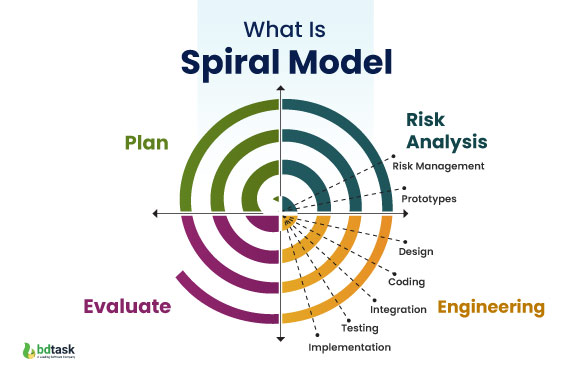
\includegraphics{assets/spiral_model.jpg}

تمام توضیحاتی که بالاتر دادیم را مدلی به نام مدل توسعه مارپیچی دارا است. این مدل در سیستم های مدرن مدیریتی برای سازماندهی تسک ها استفاده می‌شود.
با اینکار تیم های مختلف از هم فیدبک دارند و تداخلات کمتر خواهد شد. از طرفی تیم معماری با برسی و شناخت بازار به مرور فیچر های خود را به سیستم تزریق می‌کند.
بعد از انتخاب این مدل، باید به دنبال یک متدلوژی مناسب برای توسعه نرم افزار باشیم.
